\documentclass{article}
\usepackage{listings}
\usepackage{graphicx}
\usepackage{color}

\definecolor{mygreen}{rgb}{0,0.6,0}
\definecolor{mygray}{rgb}{0.5,0.5,0.5}
\definecolor{mymauve}{rgb}{0.58,0,0.82}

\lstset{ %
  backgroundcolor=\color{white},   % choose the background color; you must add \usepackage{color} or \usepackage{xcolor}; should come as last argument
  basicstyle=\footnotesize,        % the size of the fonts that are used for the code
  breakatwhitespace=false,         % sets if automatic breaks should only happen at whitespace
  breaklines=true,                 % sets automatic line breaking
  captionpos=b,                    % sets the caption-position to bottom
  commentstyle=\color{mygreen},    % comment style
  deletekeywords={...},            % if you want to delete keywords from the given language
  escapeinside={\%*}{*)},          % if you want to add LaTeX within your code
  extendedchars=true,              % lets you use non-ASCII characters; for 8-bits encodings only, does not work with UTF-8
  frame=single,	                   % adds a frame around the code
  keepspaces=true,                 % keeps spaces in text, useful for keeping indentation of code (possibly needs columns=flexible)
  keywordstyle=\color{blue},       % keyword style
  language=Octave,                 % the language of the code
  morekeywords={*,...},           % if you want to add more keywords to the set
  numbers=left,                    % where to put the line-numbers; possible values are (none, left, right)
  numbersep=5pt,                   % how far the line-numbers are from the code
  numberstyle=\tiny\color{mygray}, % the style that is used for the line-numbers
  rulecolor=\color{black},         % if not set, the frame-color may be changed on line-breaks within not-black text (e.g. comments (green here))
  showspaces=false,                % show spaces everywhere adding particular underscores; it overrides 'showstringspaces'
  showstringspaces=false,          % underline spaces within strings only
  showtabs=false,                  % show tabs within strings adding particular underscores
  stepnumber=2,                    % the step between two line-numbers. If it's 1, each line will be numbered
  stringstyle=\color{mymauve},     % string literal style
  tabsize=2,	                   % sets default tabsize to 2 spaces
  title=\lstname                   % show the filename of files included with \lstinputlisting; also try caption instead of title
}

\author{Jacob Hutter}
\title{ECE 311 Lab 7}

\begin{document}
\maketitle

\begin{figure}[H]
\color{red}
\underline{\textbf{Report Item 1}}
\color{black}
\lstinputlisting[language=Matlab]{report1.m}
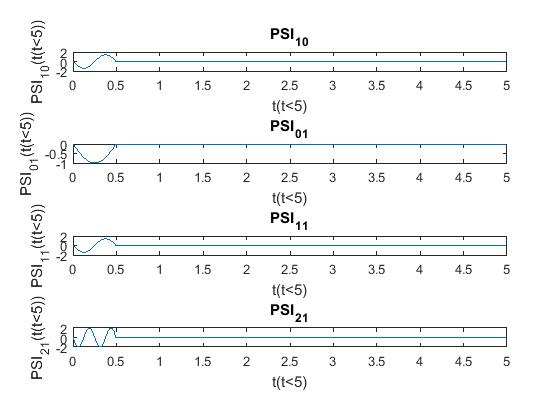
\includegraphics[scale=.5]{1}
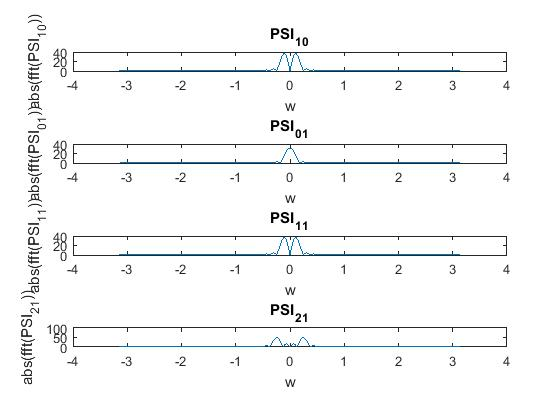
\includegraphics[scale=.5]{1_magnitude}
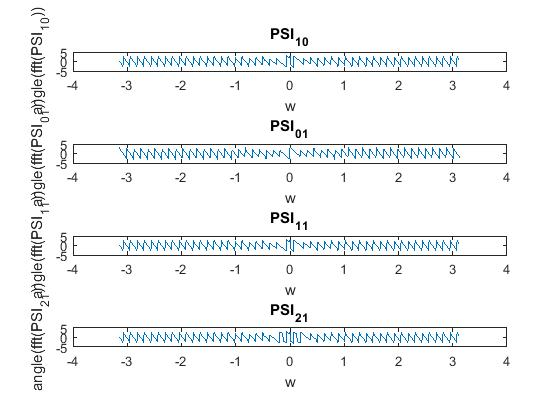
\includegraphics[scale=.5]{1_phase}
\end{figure}

\begin{figure}[H]
\color{red}
\underline{\textbf{Report Item 2}}
\color{black}
The father wavelet is called a corking function because it fills up the holes of the lower frequency components that the mother wavelets do not detect. The wavelet coeffiecients are different than fourier coefficients because in wavelet analysis, a short modulated window is used to complete
the spectral representation for that chunk. After that, the window is shifted along the signal. It is a time-frequency analysis instead a purely frequency analysis.
\end{figure}


\begin{figure}[H]
\color{red}
\underline{\textbf{Report Item 3}}
\color{black}
\lstinputlisting[language=Matlab]{report2.m}
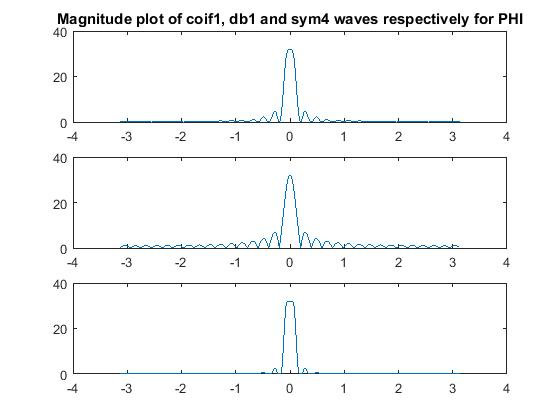
\includegraphics[scale=.5]{2_phi}
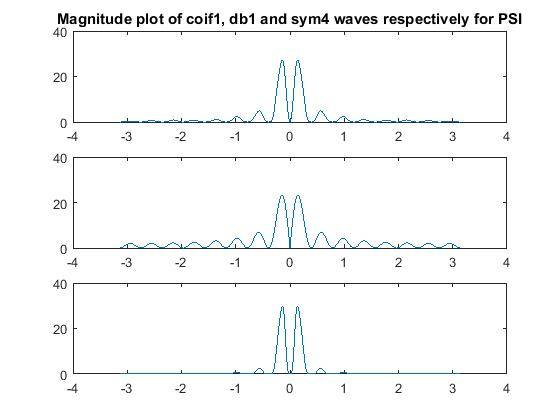
\includegraphics[scale=.5]{2_psi}
\end{figure}

\begin{figure}[H]
\color{red}
\underline{\textbf{Report Item 4}}
\color{black}
\lstinputlisting[language=Matlab]{report3.m}
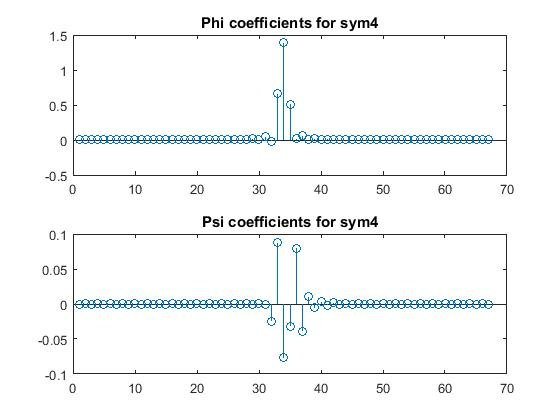
\includegraphics[scale=.5]{3_sym4}
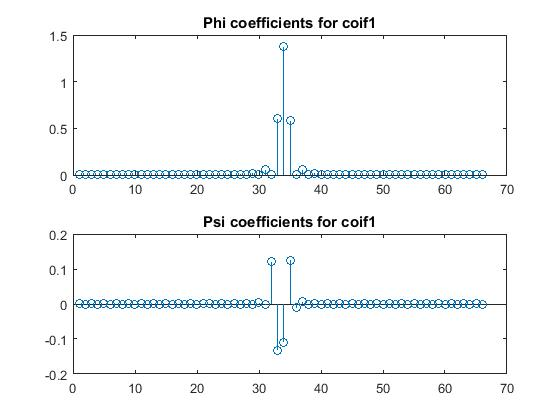
\includegraphics[scale=.5]{3_coif1}
\end{figure}

\begin{figure}[H]
\color{red}
\underline{\textbf{Report Item 5}}
\color{black}
\lstinputlisting[language=Matlab]{report4.m}
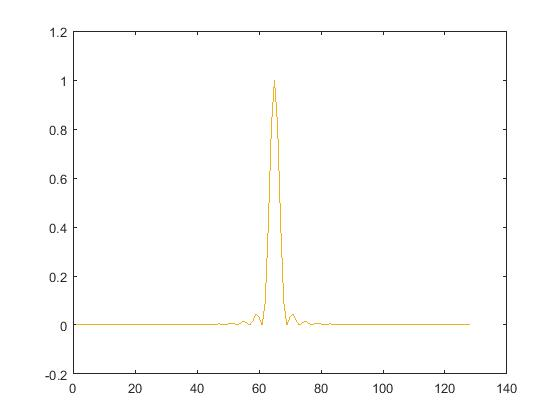
\includegraphics[scale=.5]{4_same}
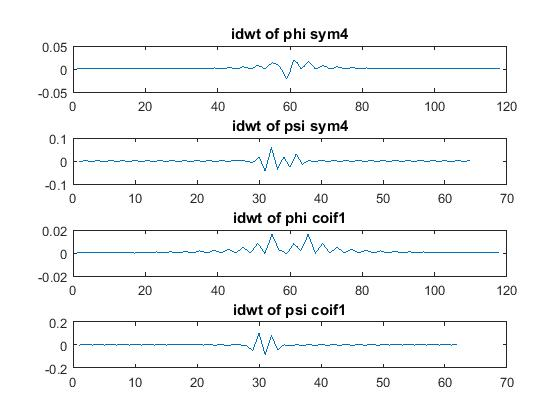
\includegraphics[scale=.5]{4_idwt}
\end{figure}

\begin{figure}[H]
\color{red}
\underline{\textbf{Report Item 6}}
\color{black}
\lstinputlisting[language=Matlab]{report5.m}
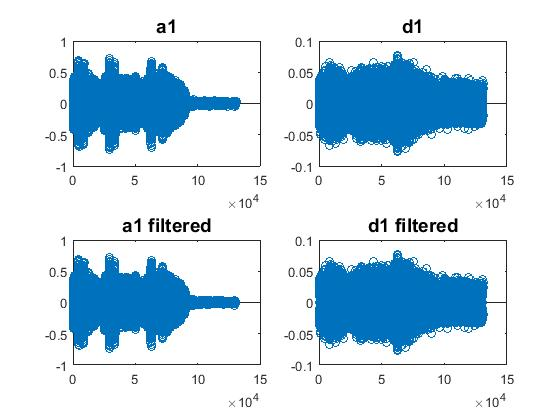
\includegraphics[scale=.5]{a1d1}
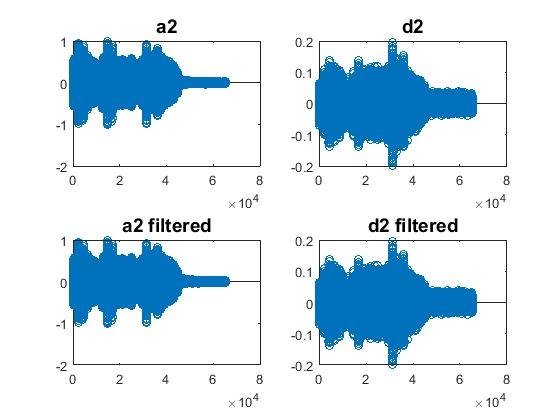
\includegraphics[scale=.5]{a2d2}
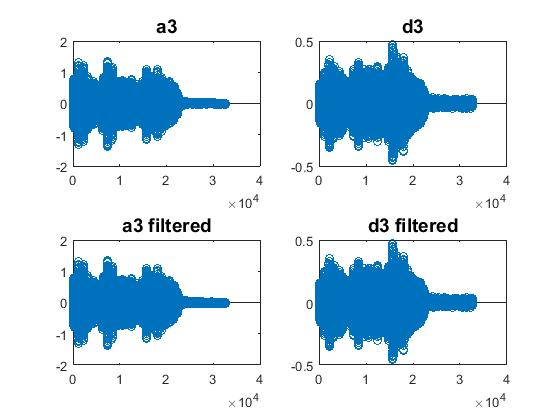
\includegraphics[scale=.5]{a3d3}
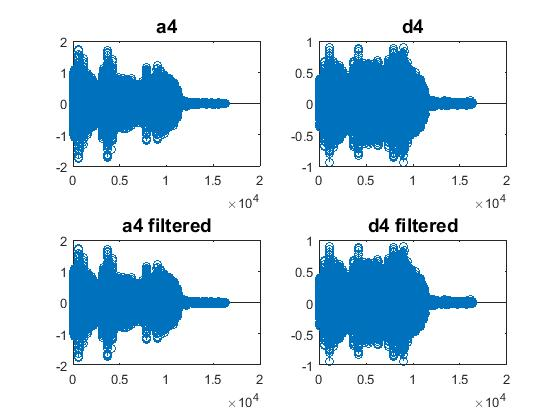
\includegraphics[scale=.5]{a4d4}
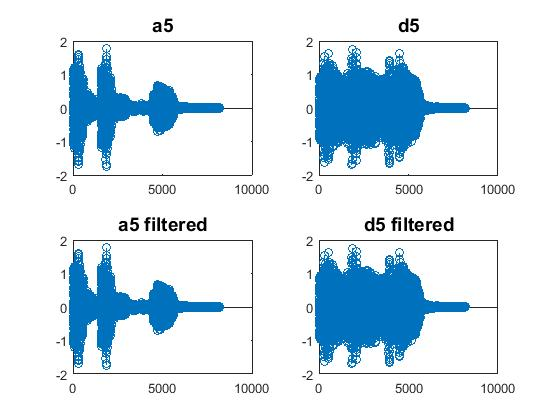
\includegraphics[scale=.5]{a5d5}
\end{figure}












\end{document}
